Below are the results of the low pass filter. The measured frequencies and amplitudes are then plotted on a bode plot.

\begin{adjustwidth}{-2.5 cm}{-2.5 cm}\centering\begin{threeparttable}[!htb]
        \scriptsize
        \begin{tabular}{lrrrrr}\toprule
            \textbf{Input Voltage(in V)} & \textbf{Output Voltage(in V)} & \textbf{Phase(in deg)} & \textbf{Frequency(in Hz)} & \textbf{Amplitude(in dB)} \\\midrule
            10.1                         & 10                            & -0.36                  & 50                        & -0.09                     \\
            10.1                         & 10                            & -0.36                  & 100                       & -0.09                     \\
            10.1                         & 10                            & -2.59                  & 200                       & -0.09                     \\
            10.2                         & 10                            & -6.49                  & 500                       & -0.17                     \\
            10.4                         & 10.1                          & -11.8                  & 1000                      & -0.25                     \\
            10.9                         & 10                            & -23                    & 2000                      & -0.75                     \\
            12.2                         & 8                             & -47.4                  & 5000                      & -3.67                     \\
            11.8                         & 5.04                          & -64                    & 10000                     & -7.39                     \\
            12.4                         & 2.8                           & -75.3                  & 20000                     & -12.93                    \\
            11.8                         & 1.14                          & -82.8                  & 50000                     & -20.30                    \\
            11.8                         & 0.596                         & -84.6                  & 100000                    & -25.93                    \\
            \bottomrule
        \end{tabular}
        \caption{The measured frequencies and amplitudes from the low pass filter.}
    \end{threeparttable}\end{adjustwidth}

The measured amplitude in decibels is found by using the relation:
\begin{equation}
    |A_{dB}| = 20\log_{10}\left(\frac{V_{out}}{V_{in}}\right)
\end{equation}


\begin{figure}[H]
    \centering
    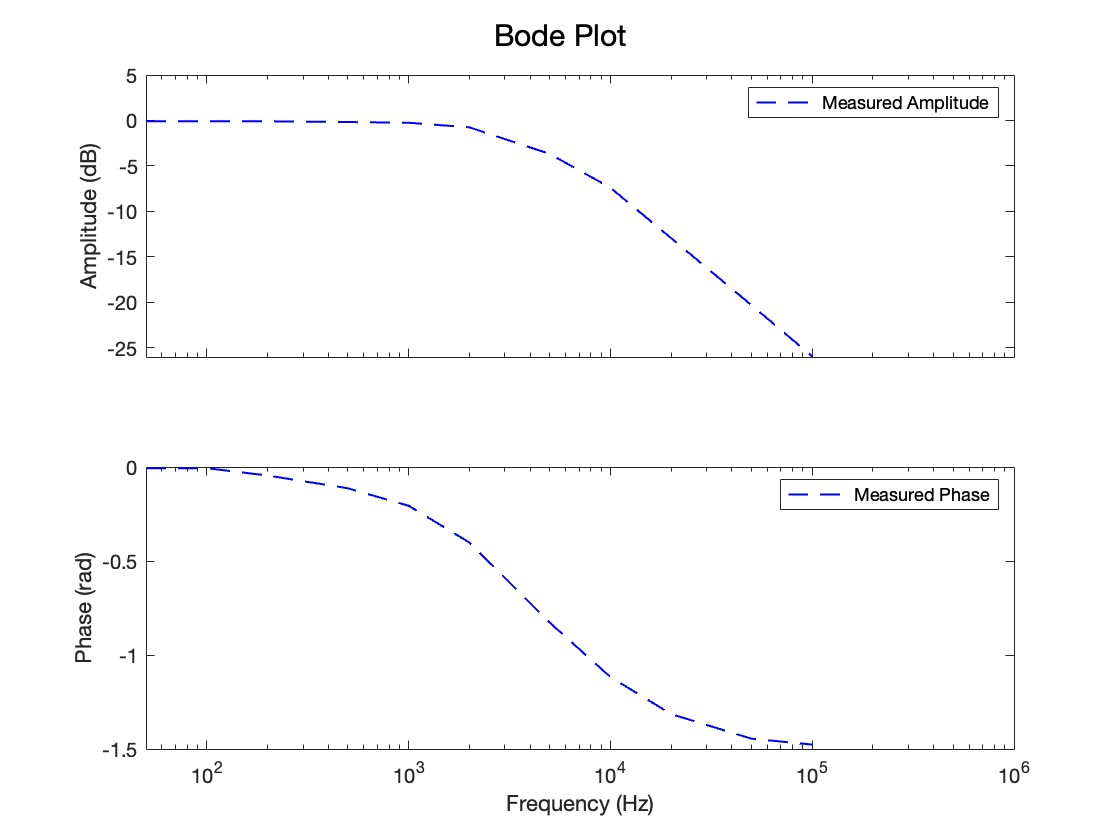
\includegraphics[scale=0.3]{images/bode_plot_low_pass_measured.jpg}
    \caption{Bode plot of measured frequencies, amplitudes and phase shifts of the low pass filter.}
\end{figure}

To draw the bode plot of the calculated amplitudes and phase, we use the following formulas:
$|\underline{A}| = \frac{1}{\sqrt{1 + (\omega RC)^2}} \text{ and } \phi = -\arctan(\omega RC)$

\begin{adjustwidth}{-2.5 cm}{-2.5 cm}\centering\begin{threeparttable}[!htb]
        \scriptsize
        \begin{tabular}{lrrr}\toprule
            \textbf{Phase(in deg) - Calculated} & \textbf{Frequency(in Hz)} & \textbf{Amplitude(in dB) - Calculated} \\\midrule
            -0.59                               & 50                        & -0.00                                  \\
            -1.19                               & 100                       & -0.00                                  \\
            -2.37                               & 200                       & -0.01                                  \\
            -5.92                               & 500                       & -0.05                                  \\
            -11.71                              & 1000                      & -0.18                                  \\
            -22.52                              & 2000                      & -0.69                                  \\
            -46.03                              & 5000                      & -3.17                                  \\
            -64.25                              & 10000                     & -7.24                                  \\
            -76.44                              & 20000                     & -12.60                                 \\
            -84.49                              & 50000                     & -20.35                                 \\
            -87.24                              & 100000                    & -26.34                                 \\
            \bottomrule
        \end{tabular}
        \caption{The calculated frequencies and amplitudes from the low pass filter using nominal values.}
    \end{threeparttable}\end{adjustwidth}

\begin{figure}[H]
    \centering
    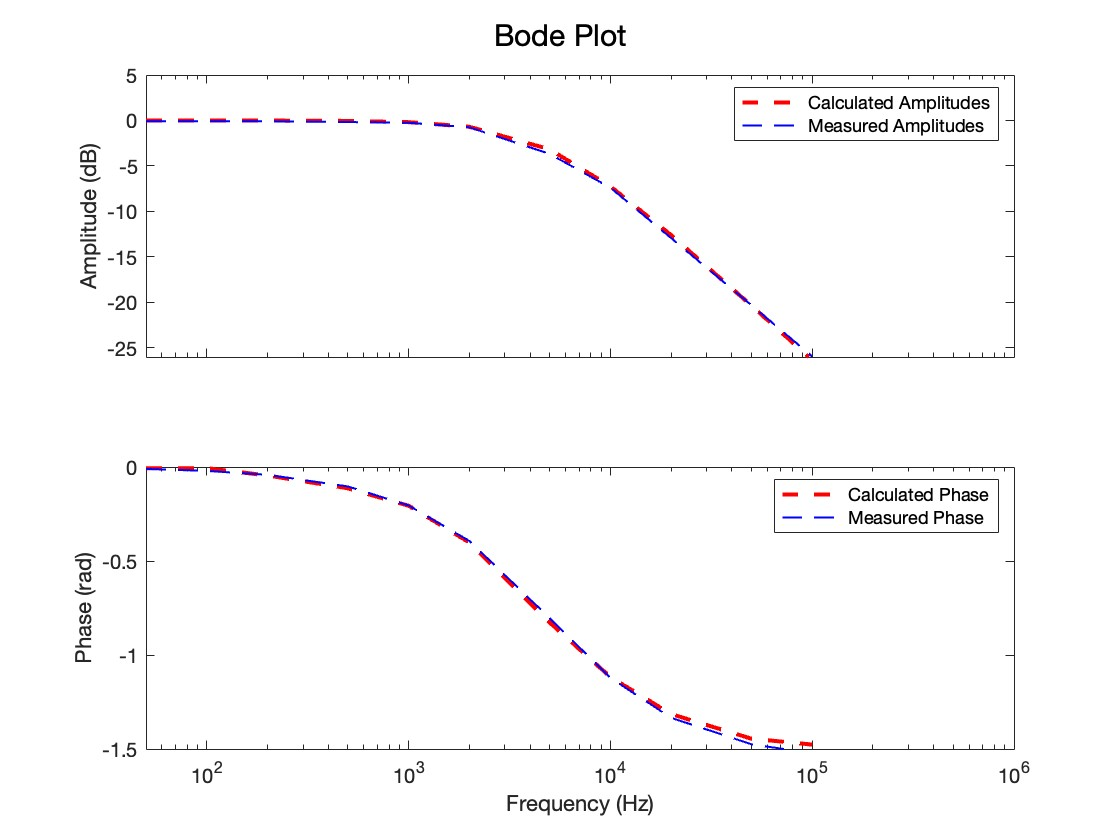
\includegraphics[scale=0.3]{images/bode_plot_low_pass_calculated.jpg}
    \caption{Bode plot of calculated amplitudes and phase shifts of the low pass filter using measured frequencies.}
\end{figure}



The calculated cutoff frequency can be obtained by the following relation for the low pass filter circuit:
\begin{equation}
    f_{-3dB} = \frac{1}{2\pi RC}
\end{equation}

Where the cutoff frequency becomes

\begin{equation}
    f_{-3dB} = \frac{1}{2\pi (22\cdot 10^3\Omega)\cdot(1\cdot 10^{-9}{F})} = 4822.8{Hz}
\end{equation}

\begin{figure}[H]
    \centering
    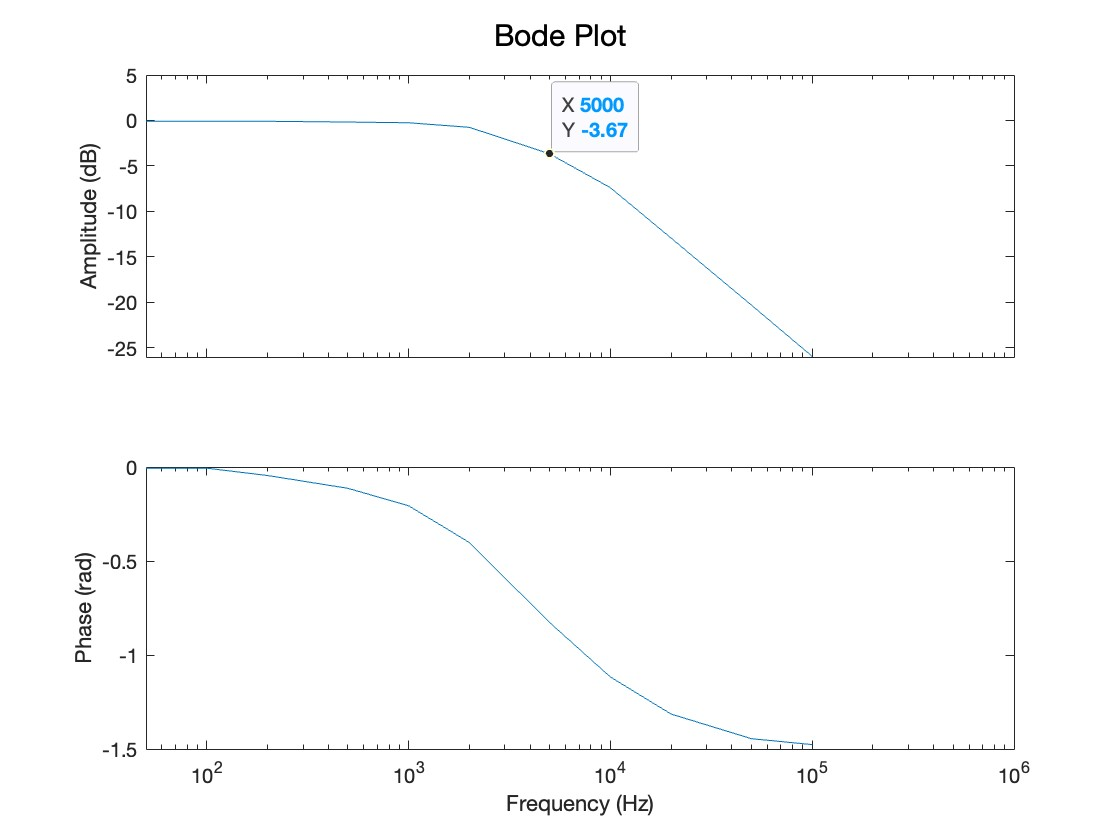
\includegraphics[scale=0.3]{images/bode_plot_low_pass_measured_cutoff.jpg}
    \caption{Bode plot of measured amplitudes and phase shifts of the low pass filter using measured frequencies.}
\end{figure}
Comparing against the cutoff frequency of the measured wave, we see that it is quite within range of the calculated cutoff frequency of 4822.8{Hz}.

To find the gradient of $|A|$ we can simply take the difference between two values. One at 100,000Hz and the other at 10,000Hz(one decade) and divide it by the logarithm of base 10 of the ratio of the frequencies(which in our case, will simply be one, as we have the unit of dB/decade).


Performing this operation, we find that:


\begin{equation}
    \frac{\Delta |A|}{\Delta \log_{10}f} = \frac{- 26.34 + 7.24}{\log_{10}(10^5/10^4)} = -19.1\text{dB/decade}
\end{equation}

Which is relatively close to the nominal value of -20dB/decade that is expected.

\break
Taking the limit of $|A| = \frac{1}{\sqrt{1+(\omega RC)^2}}$ and the limit of $\phi = -\tan^{-1}(\omega RC)$, we get the following table:

\begin{table}[!htp]\centering
    \scriptsize
    \begin{tabular}{lrrrr}\toprule
        Case             & Behaviour of f   & Amplitude            & Phase         \\\midrule
        $f \gg f_{-3dB}$ & $f \to \infty$   & $0$                  & $-90^{\circ}$ \\
        $f = f_{-3dB}$   & $f \to f_{-3dB}$ & $\frac{1}{\sqrt{2}}$ & $-45^{\circ}$ \\
        $f \ll f_{-3dB}$ & $f \to 0$        & $1$                  & $0^{\circ}$   \\
        \bottomrule
    \end{tabular}
    \caption{The behavior of the frequency depending on the case of $f_{-3dB}$}\label{tab: }
\end{table}
By this table we can infer that when the frequency is under that of the cutoff frequency, the ratio is one - the filter should ideally let the signal pass through without attenuation and any phase shift.
We can also infer that when the frequency is that of the cut-off frequency, we get the amplitude and the phase of the corner frequency.
Lastly, we can infer that when the frequency is way greater than the cut-off frequency, the amplitude is zero and the phase is $-90^{\circ}$.